
\documentclass[12pt,aspectratio=169]{beamer}

% Packages
% Shared content style for NN and NNDS. Written by Claude (2026-10-14).
%
% Everything that shared slides rely on lives here, loaded by both courses:
% colors, notation helpers and the card system. Course themes own only the
% presentation around the content (header, footer, title page, fonts, the
% \myalert color and where \SlideSource text goes). Change a definition here,
% never by redefining it in a course file, so the two courses cannot drift.

\usepackage{mathtools,amssymb,tcolorbox}
\tcbsetforeverylayer{autoparskip}

% Semantic colors
\definecolor{darkred}{rgb}{0.55,0,0}
\definecolor{darkpastelblue}{rgb}{0.47,0.62,0.8}
\definecolor{darkcerulean}{rgb}{0.03,0.27,0.49}
\definecolor{darkgreen}{rgb}{0,0.55,0}

% Figure palette (draw.io defaults)
\definecolor{titlecolor}{RGB}{245, 242, 238}
\definecolor{drawgray}{HTML}{666666}
\definecolor{drawgray_l}{HTML}{F5F5F5}
\definecolor{drawblue}{HTML}{6C8EBF}
\definecolor{drawblue_l}{HTML}{DAE8FC}
\definecolor{drawgreen}{HTML}{82B366}
\definecolor{drawgreen_l}{HTML}{D5E8D4}
\definecolor{draworange}{HTML}{D79B00}
\definecolor{draworange_l}{HTML}{FFE6CC}
\definecolor{drawyellow}{HTML}{D6B656}
\definecolor{drawyellow_l}{HTML}{FFF2CC}
\definecolor{drawred}{HTML}{B85450}
\definecolor{drawred_l}{HTML}{EA6B66}
\definecolor{drawviolet}{HTML}{9673A6}
\definecolor{drawviolet_l}{HTML}{E1D5E7}

% Notation
\newcommand{\vc}[1]{\boldsymbol{\mathbf{#1}}}
\DeclareMathOperator*{\argmax}{arg\,max}
\DeclareMathOperator*{\argmin}{arg\,min}

% Cards: blue for definitions and computable quantities, green for goals and
% stable formulations, orange for warnings and trade-offs, red for
% training-specific or problematic elements.
\tcbset{
	nndsblue/.style={colback=drawblue_l!35!white,colframe=drawblue,boxrule=0.8pt,arc=1mm},
	nndsgreen/.style={colback=drawgreen_l!35!white,colframe=drawgreen,boxrule=0.8pt,arc=1mm},
	nndsorange/.style={colback=draworange_l!35!white,colframe=draworange,boxrule=0.8pt,arc=1mm},
	nndsred/.style={colback=drawred_l!12!white,colframe=drawred,boxrule=0.8pt,arc=1mm}
}

% A card that opens with \[ would start with an empty paragraph line plus the
% display skip, leaving more room above than below (by an amount that differs
% between engines). Set that leading equation as a centered display-style line
% instead, so the space above it is the card padding, as below.
\makeatletter
\newcommand{\nndscardlead}{\futurelet\nndscard@next\nndscard@check}
% tcolorbox follows this hook with \ignorespaces; look past it.
\def\nndscard@check{\ifx\nndscard@next\ignorespaces
	\expandafter\nndscard@skip\else\expandafter\nndscard@test\fi}
\def\nndscard@skip\ignorespaces{\nndscard@test}
\newcommand{\nndscard@test}{\@ifnextchar\[{\nndscard@display}{}}
\def\nndscard@display\[#1\]{{\centering$\displaystyle#1$\par}\@ifnextchar\end{}{\vspace{\belowdisplayskip}}}
\makeatother

% Card text is ragged-right: narrow justified columns open wide word gaps,
% especially in NNDS, which never hyphenates. Fixed display spacing: when
% parallel cards share a height, stretchable skips would otherwise spread
% the content unevenly.
\tcbset{
	nndscard/.style={before upper={\raggedright
		\setlength{\abovedisplayskip}{6pt}\setlength{\belowdisplayskip}{6pt}%
		\setlength{\abovedisplayshortskip}{6pt}\setlength{\belowdisplayshortskip}{6pt}%
		\nndscardlead}},
	nndsblue/.append style={nndscard},
	nndsgreen/.append style={nndscard},
	nndsorange/.append style={nndscard},
	nndsred/.append style={nndscard}
}

% Parallel cards share a group name and get equal heights; the second argument
% (a fixed height used by older NNDS slides) is ignored.
\tcbset{courseheight/.style 2 args={equal height group=#1}}

\usepackage{mathtools}
\usepackage{hyperref}
\usepackage{setspace}
\usepackage{tikz}
\usetikzlibrary{positioning}
\usepackage{ragged2e}
\usepackage{nicematrix}
\usepackage[compatibility=false]{caption}
\usepackage[framemethod=tikz]{mdframed}


% Theme
\usetheme{metropolis}
\metroset{subsectionpage=progressbar,sectionpage=none}
\setbeamertemplate{theorems}[numbered]

\usepackage{fontspec}
\defaultfontfeatures{LetterSpace=30}
\usepackage{microtype}

% Prefer flexible inter-word spacing over splitting words across lines.
\tolerance=1
\emergencystretch=\maxdimen
\hyphenpenalty=10000
\hbadness=10000


% Code
\usepackage{listings}
% Custom colors
\definecolor{codegreen}{rgb}{0,0.6,0}
\definecolor{codegray}{rgb}{0.5,0.5,0.5}
\definecolor{codepurple}{rgb}{0.58,0,0.82}
\definecolor{backcolour}{rgb}{0.95,0.95,0.92}
\definecolor{light-gray}{gray}{0.95}
% Python style for highlighting
\newcommand\pythonstyle{\lstset{
		backgroundcolor=\color{white},
		language=Python,
		basicstyle=\ttfamily\footnotesize,
		morekeywords={self},              % Add keywords here
		keywordstyle=\color{blue},
		stringstyle=\footnotesize\color{deepgreen},
		commentstyle=\color{codegreen},
		showstringspaces=false,
		frame=tb,
		numbers=left,
		numbersep=5pt,
		numberstyle=\tiny\color{gray},
		columns=fullflexible,
		numbersep=5pt,
		aboveskip=1em,
		showtabs=false,
		tabsize=2,
		gobble=3
	}}

% Python environment
\lstnewenvironment{python}[1][]
{
	\pythonstyle
	\lstset{#1}
}
{}
% Python for inline
\newcommand\pythoninline[1]{{\pythonstyle\lstinline!#1!}}

% Tables and justification
\newcommand{\ra}[1]{\renewcommand{\arraystretch}{#1}}
\justifying

% Subfigures
\setbeamertemplate{caption}[numbered]
\usepackage[caption=false,font=footnotesize]{subfig}

% Colors
\setbeamercolor{uppercolgreen}{fg=white,bg=green!35}
\setbeamercolor{lowercolgreen}{fg=black,bg=green!10}
\setbeamercolor{uppercolred}{fg=white,bg=red!35}
\setbeamercolor{lowercolred}{fg=black,bg=red!10}
\setbeamercolor{uppercolblue}{fg=white,bg=blue!35}
\setbeamercolor{lowercolblue}{fg=black,bg=blue!10}
\definecolor{deepblue}{rgb}{0,0,0.5}
\definecolor{deepred}{rgb}{0.6,0,0}
\definecolor{deepgreen}{rgb}{0,0.5,0}

% Matrix size
\usepackage{stackengine}
\stackMath
\def\sss{\scriptstyle \color{gray}}
\setstackgap{L}{12pt}
\def\stacktype{L}

% Mathematical commands
\newcommand{\pr}[1]{{#1\,}'}
\newcommand{\idx}[2]{{\color{darkpastelblue}[}#1{\color{darkpastelblue}]_{#2}}}
\newcommand{\shape}[2]{\stackunder{#1}{\sss #2}}

% Style commands
\newcommand{\myalert}[1]{{\color{darkred}\textbf{#1}}}

% White background on every slide, so figures with a white canvas blend in
% (Simone, 2026-10-14). whiteframe is kept as an alias for existing slides.
\setbeamercolor{background canvas}{bg=white}

% White frame (for images)
\newenvironment{whiteframe}[1]{
	\setbeamercolor{background canvas}{bg=white}
	\begin{frame}{#1}
		}{
	\end{frame}
}

\setbeamerfont{frametitle}{size=\normalsize}
\setbeamertemplate{frametitle}[default][right]
% Slimmer header, close to NN's share of the slide height (Simone, 2026-10-14).
\makeatletter
\patchcmd{\beamer@@tmpl@frametitle}{sep=0.3cm}{sep=0.2cm}{}{\PackageWarning{style}{frametitle padding not patched}}
\makeatother
{
}
%\setbeamercolor{frametitle}{fg=white,bg=black!75}

% No headline frame
\makeatletter
\newenvironment{noheadline}{
	\setbeamertemplate{headline}{}
	\addtobeamertemplate{frametitle}{\vspace*{-3.5\baselineskip}}{}
}{}
\makeatother

% Lists
\setbeamertemplate{itemize items}[triangle]

% Footnotes
\setbeamertemplate{footnote}%
{%
	\parindent 1.5em\noindent%
	\justifying\setstretch{0.7}%
	\hbox to 1em{\hfil\insertfootnotemark}\begin{scriptsize}\insertfootnotetext\end{scriptsize}\par%
}

% Footnote without number
\newcommand\blfootnote[1]{%
	\begingroup
	\renewcommand\thefootnote{}\footnote[frame]{\noindent#1}%
	\addtocounter{footnote}{-1}%
	\endgroup
}

% Slide sources: set in the frame footer beside the page number, so they
% take no room from the content. Zero height keeps the footline unchanged.
% Global, because the footline is typeset outside the frame's group; each
% frame starts empty.
\newcommand{\insertslidesource}{}
\newcommand{\SlideSource}[1]{\gdef\insertslidesource{#1}}
\AddToHook{env/frame/begin}{\gdef\insertslidesource{}}
\setbeamertemplate{frame footer}{%
	\ifx\insertslidesource\empty\else
		\smash{\parbox[b]{0.88\textwidth}{\raggedright\scriptsize\color{black!60}\insertslidesource}}%
	\fi}

% Theorems
\newcommand*{\theorembreak}{\usebeamertemplate{theorem end}\framebreak\usebeamertemplate{theorem begin}}
\newcounter{theo}[section]\setcounter{theo}{0}
\renewcommand{\thetheo}{\arabic{section}.\arabic{theo}}

\newenvironment{theo}[2][]{%
	\refstepcounter{theo}%
	\ifstrempty{#1}%
	{\mdfsetup{%
			frametitle={%
					\tikz[baseline=(current bounding box.east),outer sep=0pt]
					\node[anchor=east,rectangle,fill=red!10]
					{\strut Theorem~\thetheo};}}
	}%
	{\mdfsetup{%
			frametitle={%
					\tikz[baseline=(current bounding box.east),outer sep=0pt]
					\node[anchor=east,rectangle,fill=red!10]
					{\strut Theorem~\thetheo:~#1};}}%
	}%
	\mdfsetup{innertopmargin=5pt,linecolor=red!10,%
		linewidth=2pt,topline=true,%
		frametitleaboveskip=\dimexpr-\ht\strutbox\relax
	}
	\begin{mdframed}[]\relax%
		\label{#2}}{\end{mdframed}}

\usetikzlibrary{arrows.meta,calc}
\graphicspath{{assets/}{../../shared/assets/}}
\newcommand*{\boldone}{\text{\usefont{U}{bbold}{m}{n}1}}

\usepackage{annotate-equations}
\usepackage{subfig}

% Colors
\definecolor{titlecolor}{RGB}{245, 242, 238} 
\definecolor{drawgray}{HTML}{666666}
\definecolor{drawgray_l}{HTML}{F5F5F5}
\definecolor{drawblue}{HTML}{6C8EBF}
\definecolor{drawblue_l}{HTML}{DAE8FC}
\definecolor{drawgreen}{HTML}{82B366}
\definecolor{drawgreen_l}{HTML}{D5E8D4}
\definecolor{draworange}{HTML}{D79B00}
\definecolor{draworange_l}{HTML}{FFE6CC}
\definecolor{drawyellow}{HTML}{D6B656}
\definecolor{drawyellow_l}{HTML}{FFF2CC}
\definecolor{drawred}{HTML}{B85450}
\definecolor{drawred_l}{HTML}{EA6B66}
\definecolor{drawviolet}{HTML}{9673A6}
\definecolor{drawviolet_l}{HTML}{E1D5E7}

\begin{document}

	{\usebackgroundtemplate{\tikz\node[opacity=0.4,inner sep=0]{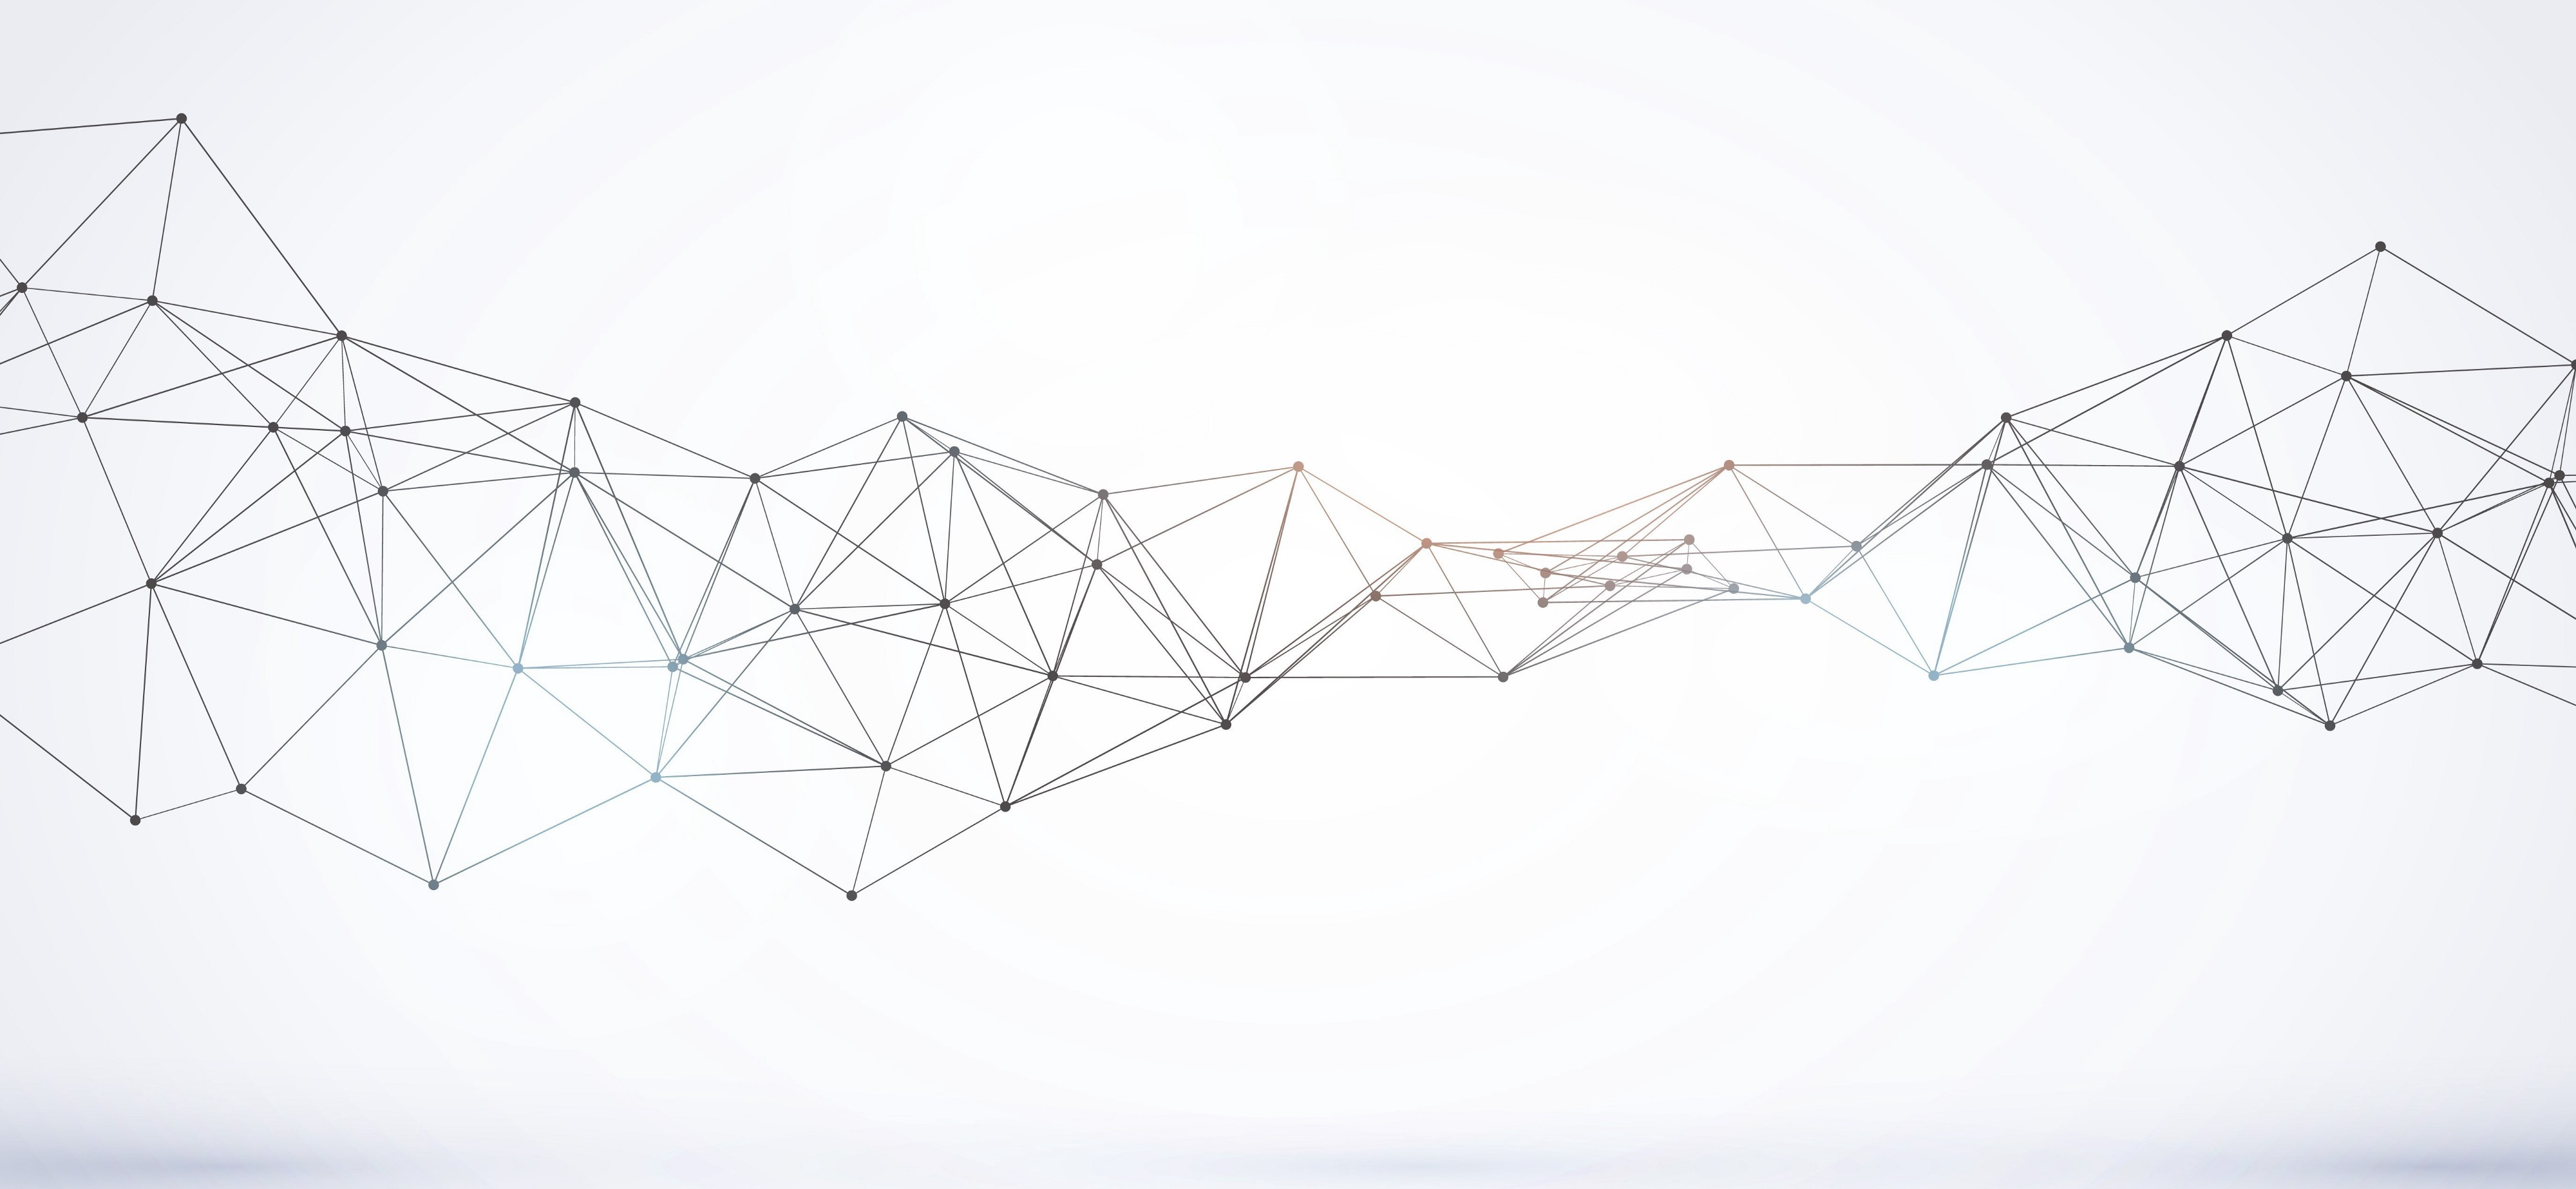
\includegraphics[width=\paperwidth,height=\paperheight]{images/header}};}%
	\begin{frame}[plain]
		\vspace{0.5cm}
		\title{\large \begin{spacing}{1.0}Neural Networks for Data Science\end{spacing}\vspace{0.25em}
			\normalsize \begin{spacing}{1.0}\textbf{Master's Degree in Data Science}\end{spacing}\vspace{0.5em}}
		\subtitle{\Large \textbf{Convolutional neural networks}}
		\date{
			{
\includegraphics[scale=0.8]{images/Uniroma1}}
		}
		\author{
			\setlength{\tabcolsep}{2pt}
			\begin{tabular}{rl}
				\textbf{Lecturer}: & S. Scardapane \\
			\end{tabular}
		}\titlepage
	\end{frame}
	}

\part{1}

\section{Introduction}
\subsection{Why fully-connected layers are not enough}

\begin{frame}{Definition of an image}
	
	An \myalert{image} is a $3$-dimensional tensor $\stackunder{X}{\sss (h,w,c)}$, where:
	%
	\begin{itemize}
		\item $h$ is the \textbf{height} of the image (e.g., 512 pixels).
		\item $w$ is the \textbf{width} of the image (e.g., 1024 pixels).
		\item $c$ is the number of \textbf{channels} (e.g., $3$ channels for a RGB image, $1$ channel for a greyscale image).
	\end{itemize}
	%
	The first two dimensions have a precise \textit{grid} ordering, while the channels do not have a precise ordering (i.e., we can switch RGB to GBR or BRG with no information loss).
	
\end{frame}

\begin{frame}{An MLP at every pixel}

    As we saw for sequences, we can apply the same MLP at every pixel:
    \[
        \idx{H}{i,j,:} = f_{\boldsymbol{\theta}}(\idx{X}{i,j,:}),
        \qquad H \sim (h,w,c').
    \]

    Each pixel is processed independently. The MLP mixes channels, but does
    not use the neighboring pixels.

    The same parameters are shared across all locations, so the number of
    parameters does not depend on the size of the image.

    How can we also exchange information between pixels?

\end{frame}

\begin{frame}{Vectorizing an image}

    A simple way to process the whole image is to \myalert{vectorize} it,
    apply a fully-connected layer, and reshape the output:
    \[
        \shape{\vc{x}}{(hwc)} = \operatorname{vect}(X),
        \qquad
        H = \operatorname{unvect}\!\left(\phi(\vc{W}\vc{x}+\vc{b})\right).
    \]

    We can choose the output shape to be $(h,w,c')$, so that the layer can
    be composed with other image layers.

    Now every output pixel can depend on the entire image. However, the
    weight matrix has $hwc \cdot hwc'$ parameters. Nothing in this layer
    forces it to use the spatial structure of the image.

\end{frame}

\begin{frame}{Two ways to process an image}
    \centering
    \scalebox{0.97}{% Editable CNN comparison: which input pixels one output pixel depends on,
% for a positionwise MLP and for a fully-connected layer on the vectorized image.
% Redrawn by Claude (2026-10-15) after Simone's review ("too basic").
\begingroup
% #1,#2: lower-left corner; #3: 1 = only the centre pixel is used,
% 2 = every pixel is used, 0 = output grid (centre pixel highlighted).
\newcommand{\cnnPixelGrid}[3]{%
    \begin{scope}[shift={(#1,#2)}]
        % two offset layers suggest the channel axis
        \foreach \k in {2,1}{
            \fill[drawgray_l] (0.12*\k,0.12*\k) rectangle ++(1.65,1.65);
            \draw[drawgray!45,line width=0.4pt] (0.12*\k,0.12*\k) rectangle ++(1.65,1.65);
        }
        \foreach \row in {0,1,2}{
            \foreach \col in {0,1,2}{
                \pgfmathtruncatemacro{\centre}{(\row==1)&&(\col==1)}
                \ifnum#3=2
                    \fill[drawblue_l] (0.55*\col,0.55*\row) rectangle ++(0.55,0.55);
                \else
                    \fill[white] (0.55*\col,0.55*\row) rectangle ++(0.55,0.55);
                    \ifnum\centre=1
                        \ifnum#3=1
                            \fill[drawblue_l] (0.55*\col,0.55*\row) rectangle ++(0.55,0.55);
                        \else
                            \fill[drawgreen_l] (0.55*\col,0.55*\row) rectangle ++(0.55,0.55);
                        \fi
                    \fi
                \fi
                \draw[drawgray!70,line width=0.4pt] (0.55*\col,0.55*\row) rectangle ++(0.55,0.55);
            }
        }
        \ifnum#3=0
            \draw[drawgreen,line width=1.1pt] (0.55,0.55) rectangle ++(0.55,0.55);
        \else
            \ifnum#3=1
                \draw[drawblue,line width=1.1pt] (0.55,0.55) rectangle ++(0.55,0.55);
            \else
                \draw[drawblue,line width=1.1pt] (0,0) rectangle ++(1.65,1.65);
            \fi
        \fi
    \end{scope}
}

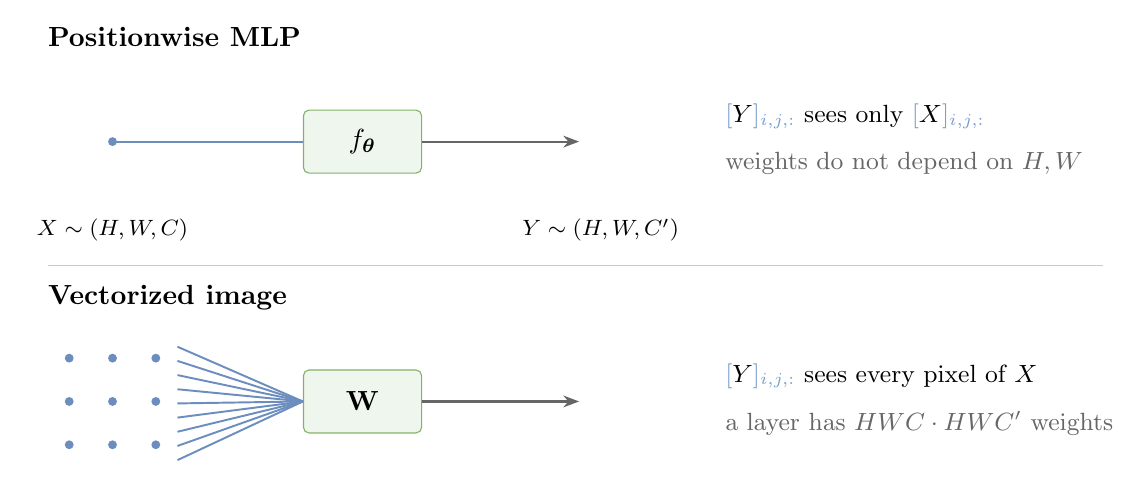
\begin{tikzpicture}[x=1cm,y=1cm,
    block/.style={draw=drawgreen,fill=drawgreen_l!40!white,rounded corners=2pt,
        minimum width=1.5cm,minimum height=0.8cm,inner sep=3pt,font=\normalsize},
    wire/.style={drawblue,line width=0.7pt},
    edge/.style={-{Stealth[length=2mm]},line width=0.8pt,draw=drawgray},
    heading/.style={font=\normalsize\bfseries,anchor=west,inner sep=0pt},
    note/.style={font=\small,anchor=west,align=left,inner sep=0pt}]

% ---- Positionwise MLP: one input pixel per output pixel
\node[heading] at (0,5.05) {Positionwise MLP};
\cnnPixelGrid{0}{2.9}{1}
\cnnPixelGrid{6.2}{2.9}{0}
\node[block] (pw) at (4.0,3.725) {$f_{\boldsymbol{\theta}}$};
\fill[drawblue] (0.825,3.725) circle (1.6pt);
\draw[wire] (0.825,3.725) -- (1.65,3.725) -- (pw.west);
\draw[edge] (pw.east) -- (6.75,3.725);
\node[font=\footnotesize] at (0.825,2.6) {$X\sim(H,W,C)$};
\node[font=\footnotesize] at (7.025,2.6) {$Y\sim(H,W,C')$};
\node[note] at (8.6,4.05) {$\idx{Y}{i,j,:}$ sees only $\idx{X}{i,j,:}$};
\node[note,text=drawgray] at (8.6,3.45) {weights do not depend on $H,W$};

\draw[drawgray!35,line width=0.5pt] (0,2.15)--(13.4,2.15);

% ---- Vectorized image: every input pixel for every output pixel
\node[heading] at (0,1.75) {Vectorized image};
\cnnPixelGrid{0}{-0.4}{2}
\cnnPixelGrid{6.2}{-0.4}{0}
\node[block] (fc) at (4.0,0.425) {$\vc{W}$};
% one wire per pixel, fanning out from the right edge of the grid
\foreach \row in {0,1,2}{
    \foreach \col in {0,1,2}{
        \fill[drawblue] (0.275+0.55*\col,-0.125+0.55*\row) circle (1.6pt);
    }
}
\foreach \k in {0,...,8}{
    \draw[wire] (1.65,-0.32+0.18*\k) -- (fc.west);
}
\draw[edge] (fc.east) -- (6.75,0.425);
\node[note] at (8.6,0.75) {$\idx{Y}{i,j,:}$ sees every pixel of $X$};
\node[note,text=drawgray] at (8.6,0.15) {a layer has $HWC\cdot HWC'$ weights};
\end{tikzpicture}
\endgroup
}
\end{frame}

\begin{frame}{An example to keep in mind}
\small
\setlength{\parskip}{2pt}
\setlength{\arraycolsep}{7pt}
\setlength{\abovedisplayskip}{5pt}
\setlength{\belowdisplayskip}{5pt}

	As a running example to visualize what follows, consider a 1D sequence (think of this as “\textit{4 pixels with a single channel}”):

	$$
	\mathbf{x} = \left[x_1, x_2, x_3, x_4\right]
	$$
	
	In this case, we do not need any reshaping operations, and the previous layer (with $c^\prime = 1$) can be written as:
	
	$$
	\begin{bmatrix} h_1 \\ h_2 \\ h_3 \\ h_4 \end{bmatrix}=\begin{bmatrix}W_{11} & W_{12} & W_{13} & W_{14} \\ W_{21} & W_{22} & W_{23} & W_{24} \\ W_{31} & W_{32} & W_{33} & W_{34} \\ W_{41} & W_{42} & W_{43} & W_{44} \end{bmatrix} \begin{bmatrix} x_1 \\ x_2 \\ x_3 \\ x_4 \end{bmatrix}
	$$

\end{frame}

\section{Convolutional neural networks}
\subsection{Convolutional layers}

% Written by Codex (2026-10-13): convolutional-layers review candidate.
\begin{whiteframe}{Local neighborhoods}

    \begin{columns}[c,onlytextwidth]
        \begin{column}{0.54\textwidth}
            With a \myalert{kernel size} $s=2k+1$, we take the $s \times s$
            neighborhood centered at $(i,j)$, including all $c$ channels.

            We write this local tensor as:
            \[
                P_k(i,j) \sim (s,s,c).
            \]
        \end{column}
        \begin{column}{0.42\textwidth}
            \centering
            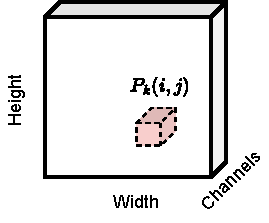
\includegraphics[width=\linewidth,height=0.46\textheight,keepaspectratio]{images/cnn/book/patch.pdf}
        \end{column}
    \end{columns}

    \vspace{0.5em}
    \begin{tcolorbox}
        A layer is \myalert{local} if $\idx{H}{i,j,:}$ depends only on $P_k(i,j)$.
    \end{tcolorbox}

\end{whiteframe}

\begin{frame}{Convolutional layer}

    We apply the same affine map and activation to every neighborhood:
    \[
        \idx{H}{i,j,:}
        = \phi\!\left(
            {\color{darkgreen}\vc{W}^{\top}}\,
            \shape{\operatorname{vect}(P_k(i,j))}{(s^2c)}
            + {\color{darkcerulean}\vc{b}}
        \right).
    \]

    We share the weights $\vc{W} \sim (s^2c,c')$ and bias $\vc{b} \sim (c')$
    \textbf{across all locations}.

    This is a \myalert{convolutional layer}. It has $s^2cc' + c'$ parameters,
    regardless of the image height and width.

    The convolution is the affine map inside the parentheses. We apply
    the usual pointwise activation $\phi$ to its output.

\end{frame}

\begin{whiteframe}{Filters and output channels}

    Each column of $\vc{W}$ defines a \myalert{filter}, producing one output
    channel. A spatial slice $\idx{H}{:,:,a}$ is an \myalert{activation map}.

    \begin{figure}
        \centering
        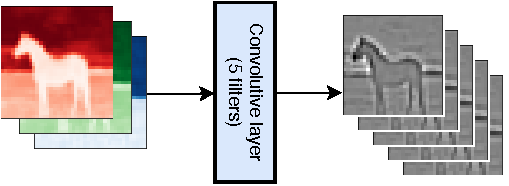
\includegraphics[width=0.7\columnwidth]{images/cnn/source/Convolutive_layer.pdf}
    \end{figure}

\end{whiteframe}

\begin{frame}{Zero-padding}
    \setlength{\parskip}{3pt}
    \setlength{\abovedisplayskip}{9pt}
    \setlength{\belowdisplayskip}{9pt}

    For our four-element sequence, a size-$3$ kernel produces only two outputs
    without padding. We add one zero at each end to obtain four outputs:
    \[
        \widetilde{\vc{x}}
        = \begin{bmatrix}
            {\color{darkcerulean}0} & x_1 & x_2 & x_3 & x_4 & {\color{darkcerulean}0}
          \end{bmatrix}^{\top}.
    \]

    With \myalert{zero padding}, we treat values outside the input as zero.

    \begin{tcolorbox}
        For an odd kernel size $s$, we add $k=(s-1)/2$ zeros at each end to
        preserve the input length when evaluating every position.
    \end{tcolorbox}

    In 2D, we pad each border with $k$ rows or columns: one for a $3 \times 3$
    kernel, two for a $5 \times 5$ kernel.

\end{frame}

\begin{frame}{Running example}
    \setlength{\arraycolsep}{7pt}

    We apply a size-$3$ kernel to the padded sequence, without bias or activation:
    \[
        \begin{bmatrix} h_1 \\ h_2 \\ h_3 \\ h_4 \end{bmatrix}
        =
        \begin{bmatrix}
            {\color{darkgreen}W_1} & {\color{darkgreen}W_2} & {\color{darkgreen}W_3} & 0 & 0 & 0 \\
            0 & {\color{darkgreen}W_1} & {\color{darkgreen}W_2} & {\color{darkgreen}W_3} & 0 & 0 \\
            0 & 0 & {\color{darkgreen}W_1} & {\color{darkgreen}W_2} & {\color{darkgreen}W_3} & 0 \\
            0 & 0 & 0 & {\color{darkgreen}W_1} & {\color{darkgreen}W_2} & {\color{darkgreen}W_3}
        \end{bmatrix}
        \begin{bmatrix}
            {\color{darkcerulean}0} \\ x_1 \\ x_2 \\ x_3 \\ x_4 \\ {\color{darkcerulean}0}
        \end{bmatrix}.
        \label{eq:convolution_example}
    \]

    This is a \myalert{Toeplitz} matrix: the weights are constant along each
    diagonal. We learn three coefficients, compared with sixteen for the
    earlier dense layer.

\end{frame}

\begin{frame}{Translation equivariance}

    Shared weights give the same response to the same neighborhood,
    wherever it appears in the image.

    We write $T_{\delta}$ for a shift by $\delta$ pixels.
    \begin{tcolorbox}
        A layer $f$ is \myalert{translation equivariant} if shifting the
        input shifts its output by the same amount:
        \[
            f(T_{\delta}X)=T_{\delta}f(X).
        \]
    \end{tcolorbox}

    For convolution evaluated at every pixel, this holds away from image
    boundaries. Zero padding can change the response near an edge.

\end{frame}

\begin{frame}{Receptive field}
    \setlength{\parskip}{3pt}

    We combine information across larger regions by stacking local layers.

    \begin{tcolorbox}
        The \myalert{receptive field} of $\idx{H}{i,j,:}$ is the region
        of the input that can affect that output.
    \end{tcolorbox}

    Away from the boundaries, $L$ layers with kernel size $s$, evaluated
    at every pixel, give a receptive field of width:
    \[
        R_L=1+L(s-1).
    \]

    With $3 \times 3$ kernels, the receptive field grows from $3 \times 3$
    to $5 \times 5$ to $7 \times 7$ over the first three layers.

\end{frame}

\begin{frame}[fragile]{Implementation}
    \setlength{\parskip}{3pt}
    \setlength{\abovedisplayskip}{7pt}
    \setlength{\belowdisplayskip}{7pt}

    We can collect flattened, padded neighborhoods as columns of $U(X)$:
    \[
        \shape{\widetilde{Z}}{(c',hw)}
        = \shape{\vc{W}^{\top}}{(c',s^2c)}\,
          \shape{U(X)}{(s^2c,hw)}
          + \vc{b}.
    \]

    \begin{python}[gobble=4,aboveskip=5pt,belowskip=5pt]
    import torch
    X = torch.randn(1, 3, 64, 64)  # (B, C, H, W)
    conv = torch.nn.Conv2d(3, 100, 5, padding=2)
    Z = conv(X)  # (1, 100, 64, 64)
    \end{python}

    In practice, \verb+nn.Conv2d+ uses a specialized implementation for the
    hardware, so we do not construct $U(X)$ explicitly. We will see more in the lab.

    \blfootnote{\href{https://docs.pytorch.org/docs/stable/generated/torch.nn.Unfold.html}{PyTorch: Unfold}
        and \href{https://docs.nvidia.com/deeplearning/performance/dl-performance-convolutional/index.html}{NVIDIA: convolution implementations}.}

\end{frame}

\subsection{Defining the network}

% Written by Codex (2026-10-14): light defining-the-network review candidate.
\begin{frame}{Reducing dimensionality}

    We can define a convolutional block by interleaving convolutions with
    activation functions:
    \[
        H = (\phi \circ \text{Conv}\circ\ldots\circ\phi\circ\text{Conv})(X).
    \]

    With the padding introduced earlier, evaluating every position preserves
    the spatial resolution $(h,w)$. These blocks can still change the number of
    channels. We can reduce the resolution between blocks to save computation
    and memory.

    This also connects to \myalert{multi-resolution} filter banks in signal
    processing, where we process a signal at different resolutions.

\end{frame}

\begin{frame}[fragile]{Stride}
    \setlength{\parskip}{3pt}
    \setlength{\abovedisplayskip}{7pt}
    \setlength{\belowdisplayskip}{7pt}

    With \myalert{stride} $r$, we move the kernel by $r$ pixels along each
    spatial axis. Using zero-based indices, we compute:
    \[
        \idx{H}{i,j,:}
        = \phi\!\left(\vc{W}^{\top}\operatorname{vect}(P_k(ri,rj))+\vc{b}\right).
    \]

    For the odd kernels with padding $k$ introduced earlier, the output has shape
    \[
        H \sim (\lceil h/r \rceil,\lceil w/r \rceil,c').
    \]
    With $r=2$, this is $(h/2,w/2,c')$ when $h$ and $w$ are even.

    In PyTorch, we set \verb+stride=2+ in \verb+nn.Conv2d+.

\end{frame}

\begin{whiteframe}{Convolution with a larger stride}

    \vspace{1.5em}
    \begin{figure}
        \centering
        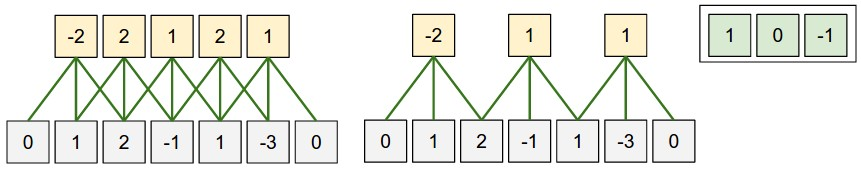
\includegraphics[width=0.95\columnwidth]{images/cnn/source/stride.jpg}
        \caption{Stride $1$ on the left, stride $2$ on the right.
            Image source: \href{https://cs231n.github.io/convolutional-networks/}{CS231n}.}
    \end{figure}

\end{whiteframe}

\begin{frame}{Max-pooling}

    We can also reduce the resolution with a \myalert{max-pooling} or
    \myalert{average-pooling} layer. We take the maximum or average over small
    windows, independently in each channel.

    We can use $2 \times 2$ or $4 \times 4$ windows.
    With a $2 \times 2$ window and stride $2$, we halve each spatial dimension
    when the input height and width are even.

\end{frame}

\begin{whiteframe}{Visualization of max-pooling}

    \vspace{1.5em}
    \begin{figure}
        \centering
        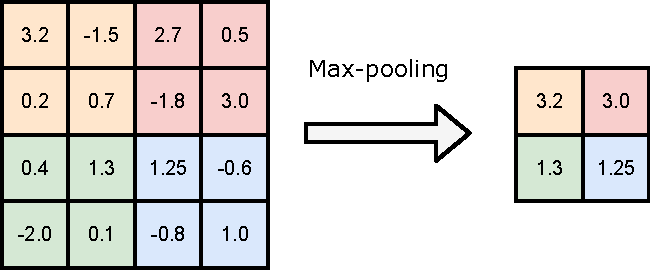
\includegraphics[width=0.7\columnwidth]{images/cnn/book/max_pooling.pdf}
        \caption{Max-pooling on a $4 \times 4$ image, with $2 \times 2$ windows
            and stride $2$. We can replace the maximum with an average or another
            differentiable aggregation.}
    \end{figure}

\end{whiteframe}

\begin{frame}{Complete architecture of a CNN (1)}
    \setlength{\parskip}{3pt}

    A standard CNN for classification combines:
    \begin{itemize}
        \item Convolutional blocks, with strided convolutions or pooling
            to reduce the resolution.
        \item Flattening or \myalert{global pooling}.
        \item A classification block.
    \end{itemize}

    Global pooling is \myalert{invariant} to shifts that only rearrange the
    feature map. Image boundaries and downsampling can prevent exact translation
    invariance of the complete CNN.

    More recent CNNs vary this basic architecture. Choosing the blocks and
    their hyperparameters remains a \textit{model selection} problem.

\end{frame}

\begin{frame}{Complete architecture of a CNN (2)}
    \setlength{\arraycolsep}{3pt}

    We choose either flattening (Block 2a) or global average pooling
    (Block 2b) before the classifier:
    \[
        \begin{array}{rclr}
            \textrm{Block 1:} & \shape{H}{(h',w',c')} = &
                (f_l \circ \ldots \circ f_2 \circ f_1)(X) &
                \text{(\color{darkred}convolution/pooling)} \\[0.8em]
            \textrm{Block 2a:} & \shape{\vc{h}}{(h'w'c')} = &
                \operatorname{vect}(H) & \text{(\color{darkgreen}flattening)} \\[0.8em]
            \textrm{Block 2b:} & \shape{\vc{h}}{(c')} = &
                \frac{1}{h'w'}\sum_{i,j}\idx{H}{i,j,:} &
                \text{(\color{darkgreen}global pooling)} \\[0.8em]
            \textrm{Block 3:} & \vc{y} = &
                \operatorname{softmax}(g(\vc{h})) &
                \text{(\color{darkcerulean}e.g., logistic regression)}
        \end{array}
    \]

\end{frame}

\begin{whiteframe}{Example of a simple CNN specification}
    \setlength{\abovecaptionskip}{5pt}
    \begin{figure}
        \centering
        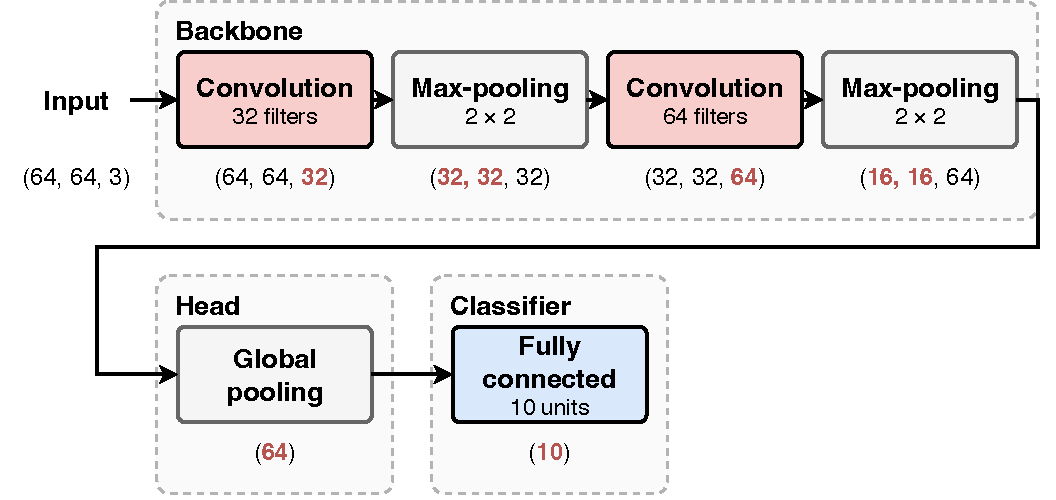
\includegraphics[width=0.79\columnwidth]{images/cnn/book/CNN_architecture.pdf}
        \caption{Pooling reduces the spatial resolution between convolutions.
            Global pooling gives one value per channel before classification.}
    \end{figure}

\end{whiteframe}

\begin{whiteframe}{Designing in blocks}

    \vspace{1em}
    \begin{figure}
        \centering
        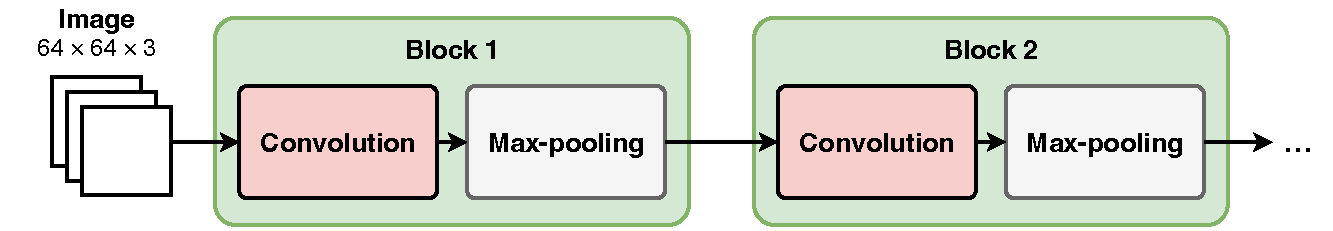
\includegraphics[width=0.8\columnwidth]{images/cnn/book/CNN_blocks.pdf}
        \caption{For deeper CNNs, we can group repeated components into
            \textit{blocks} and compose the blocks as layers.}
    \end{figure}

\end{whiteframe}

\subsection{Other notable types of convolutions}

\begin{frame}{1x1 convolutions}
	
	One important type of convolutional layer is a 1x1 layer, i.e., a layer with a kernel size of 1 ($k=0$), also called a \myalert{pointwise convolution}.
	
	This can be understood as a pixel-wise operation, which is applied independently at every pixel, with no contribution from the neighbours.
	
	It is especially important when we desire to simply modify the number of channels.
	
\end{frame}

\begin{frame}{Depth-wise convolutional layer}
	
	An orthogonal idea is to apply a convolution to each channel \textit{independently}, by combining only information across the spatial dimensions.
	
	The result is a \myalert{depth-wise} (separable) convolution:
	%
	$$
	H_{ij{\color{drawred}c}} = \sum_{i^\prime=1}^{2k+1}\sum_{j^\prime = 1}^{2k+1} W_{i^\prime, j^\prime,{\color{drawred}c}}X_{i^\prime +t(i),j^\prime+t(j),{\color{drawred}c}}
	$$
	%
	This idea can also be extended to \myalert{group} convolution. A depthwise convolution followed by a pointwise convolution is called a \myalert{depthwise-separable convolution} and it is extremely common for modeling efficient architectures.
	
\end{frame}

\begin{frame}{Further readings}
	
	\begin{itemize}
		\item \textbf{Chapter 7} of the book.
	\end{itemize}
	
\end{frame}

\end{document}
